\let\accentvec\vec
\documentclass[runningheads]{llncs}
\usepackage{array}
\usepackage{algorithm}
\usepackage{algorithmic}
\usepackage{amsmath}
\usepackage{graphicx}
\graphicspath{{./pic/}}
\let\spvec\vec
\let\vec\accentvec

\newtheorem{observation}{Observation}

\renewcommand{\algorithmicrequire}{\textbf{Input:}}   
\renewcommand{\algorithmicensure}{\textbf{Output:}}  

\linespread{1.0}
\begin{document}
	
	\title{Adaptive Online Network Intrusion Detection}
	
	\author{Yueting Chen, Vincent Chu}
	
	\institute{York University\\ 
		\email{ytchen@yorku.ca}
		\email{vwchu@my.yorku.ca}
	}
	
	\maketitle
	
	{\tiny }
	\begin{abstract} \label{abstract}
	
		Online network intrusion detection has been an important issue in both stream data mining and network security. How to identify intrusions with fast and effective algorithms is the key to most of IDS systems. In this paper, we first give an overview of online network intrusion detection systems, containing: data collection, feature extraction, normalization and online learning algorithms. We further developed a new method to detect network intrusions using classification. Two main steps are performed in the method, namely classification and data reduction. the k-NN method is applied in the classification phase while clustering techniques are introduced during data reduction. We first group records with the same labels together and keep the clusters' centers instead of raw data records. Our experiments show that our method has better accuracy compared with ECSMiner and k-NN. The influence of different values for parameters are also studied in this paper. 
		
	\end{abstract}
	
	\section{Introduction} \label{introduction}
	
	Large amount of network traffic data is generated at a rapid rate every day, since computers are everywhere in our daily life. Meanwhile, such widespread usage of the Internet also increases the potential damage that can be caused by attacks. With ever-growing proliferation of new attack methods, it is increasingly difficult to employ traditional intrusion detection methods to prevent attacks.
	
	Network intrusions are commonplace for computer networks all around the world. One recent noteworthy occurrence was the WannaCry ransom-ware attack in May 2017. This attack was estimated to have affected more than 300,000 computers in 150 countries, disruption operations in: hospitals, telecommunications, manufacturing, railways, banks, refineries, universities, and government departments as well as thousands of other organizations and businesses \cite{Cameron2017}\cite{Hern2017}\cite{Eyerys2017}. Another prominent example of network intrusion in recent years was the Sony Pictures hack of 2014, in which hackers stole and leaked to the Internet thousands of confidential documents from the film studio, including: employee personnel files, emails between employees, salary information of executives, copies of unreleased films and other sensitive information \cite{Siboni2014}. These attacks and many others highlight the importance and necessity of intrusion detection in computer networks.
	
	Intrusion detection, as an important issue in network security, has been studied for many years. Many data mining methods have already been applied to this research area, such as: neural networks, support vector machines, decision trees and so on. Most of these methods are applied on static training dataset. Thus, for every new attack type we would like to detect, we need to retrain the model again, which is inefficient and infeasible in many cases.
	
	Many data stream classification algorithms have been proposed to address two major challenges relating to data streams: infinite length and concept-drift. Data streams can run indefinitely and thus have infinite length. Therefore, a learning algorithm that requires multiple passes over a dataset would require infinite storage and training time \cite{Siboni2014}. Concept-drift, in which the underlying concept of the data changes over the time, requires that the algorithm periodically updates the model. For instance, changes in online user behaviour might result in changes to the network traffic data collected over time. These changes could impact the performance of our models if they are not updated accordingly. Some researchers have proposed some hybrid models to combine both offline and online data that address this issue \cite{Siboni2014}\cite{Masud2013}. 
	
	In this paper, we first present an overview of online network intrusion detection systems. Labels are used to identify different type of intrusions. We further propose a new online classification algorithm to improve the accuracy of results. Our technique involves both partitioning and data reduction. The rest of this paper organizes as follows: Section~\ref{related work} introduces related works. Section~\ref{Our Method} gives a detailed view of the method we proposed. Section~\ref{Experiments} then describes the data set and experiment evaluation. At last, section~\ref{conclusion} concludes with some future works that could be done.
	
	\section{Related Work} \label{related work}
	
	Our technique is related to work done in data mining based intrusion detection, online clustering, and online ensemble learning techniques.

	Intrusion detection as an application of data mining algorithm is not a new idea and there is a lot of related research in the field. There are two main categories of intrusion detection techniques: misuse detection and anomaly detection. Misuse detection uses known patterns of the malicious activity. to identify intrusions, while anomaly detection attempts to identify malicious traffic based on deviations from established normal network traffic patterns \cite{Ektefa2010}\cite{Liu2009}. In \cite{Liu2009}, the authors proposed a data mining framework for constructing intrusion detection models, based on the Apriori algorithm for association rule mining. In \cite{Ektefa2010}, the authors used classification tree and support vector machines methods to detect intrusions in network. They compared the approaches and found that the C4.5 algorithm out-performed SVM in detection and false alarm rates. In \cite{WenkeLee1999}, an approach was proposed using meta-learning as a means to construct a combined model that incorporate evidence from multiple, lightweight base models. The framework consists of various learning classifiers and meta-classifiers, association rules for link analysis, frequent episodes for sequence analysis, and an interactive, iterative environment for constructing and evaluating detection models \cite{WenkeLee1999}.

	\section{Adaptive Online Intrusion Detection} \label{Our Method}
	
	In network intrusion detection systems (IDS), raw data can be collected using online sniffing. There are many techniques that can be used to monitor the network and collect traffic logs. Raw data collected from the network can be enormous in size, since the records contain detailed information about the network traffic in binary format. Only key attributes in these record are needed for further processing. This can be done by most of network traffic analysis tools.

	In this paper, we assume that data are already collected and extracted. The data records contain attribute vectors that are sent to the IDS continuously in a streamed form.

	\subsection{Overview}
	
	\begin{figure}
		\centering
		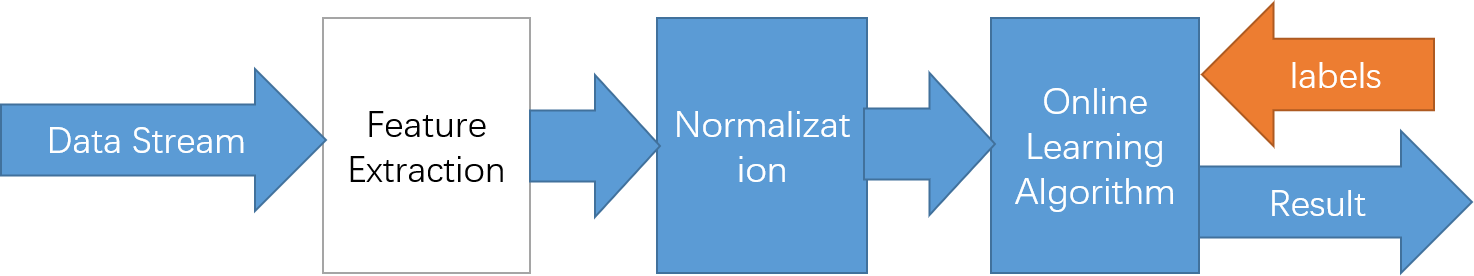
\includegraphics[width=0.8\textwidth]{overview}
		\caption{Overview of online network intrusion detection system}
		\label{fig:overview}
	\end{figure}
	
	First, an overview of our online network intrusion detection system is given in \textbf{Figure~\ref{fig:overview}}. The whole process contains three major parts, namely, feature extraction, normalization and online learning algorithm.
	
	To simplify the problem, we assume that after each classification result is reported, the correct label for that record can be obtained through user/system feedbacks. Thus, different labels can be used for various type of intrusions. Records with correct labels can be used as training stream, to further improve classification accuracy of the system online.
	
	\begin{table}
		\centering
		\caption{Summary of notations}\label{table:notation}
		\begin{tabular}{|m{1em}|m{16em}|m{1em}|m{16em}|}
			\hline
			$w$ & The maximum size of a partition & $P_i$ & A partition \\ 
			\hline
			$P$ & The set of all partitions & $N$ & Maximum number of partitions \\ 
			\hline
			$l_i$ & A label of class & $|L|$ & The number of labels  \\ 
			\hline
			$k$ & Parameter $k$ of k-NN method & $c$ & Number of clustering in K-Means \\
			\hline
		\end{tabular}
	\end{table}
	
	Table~\ref{table:notation} gives the notations that we use in the rest of this paper. Since our work is based on online data stream. A brief mathematical definition of data stream and related notations are given as follows:
	
	\begin{enumerate}
		\item \textbf{\textit{Data stream}}. A data stream is a sequence of data records in an certain arrive order: \big\{$x_1$, $x_2$, ..., $x_i$\big\}, where $x_i$ is the most recent arrived data record, and $x_1$ is the very first data record in the stream.
		\item \textbf{\textit{Data record}}. A data record in a stream contains at least two values: (1) the timestamp, which identifies the record's time of arrival; (2) the actual value of the record, specifically a vector containing different values for all the attributes.
		\item \textbf{\textit{Feedback}}. After a data record arrives, classifications can be made immediately. To simplify the problem, we assume that a correct label of the record can be obtained right after the classification process. This means when record $x_i$ arrives, the correct label of $x_{i-1}$ is already given through feedback.
	\end{enumerate}
	
	\subsection{Normalization}
	Attributes extracted from network data can have different value boundaries. In order to gain a better learning result, normalization needs to be made on incoming data stream. Not all normalization methods are suitable in online scenarios, since it is impossible to get all the statistical information before all data records are arrived. In this paper, min-max normalization is applied right after data record comes in. This is a reasonable method since most of the attributes boundaries are fixed, and can be pre-obtained from network protocols and standards.
	
	\subsection{Online Learning Algorithm}
	Many online data mining algorithms can be applied to network intrusion detection systems. In order to achieve better performance and fast speed, Trade-offs need to be made during learning phase.
	
	Algorithm~\ref{algorithm:main} gives the outline of our method. The algorithm starts with an initial set of partitions, $P$. This can be used to bootstrap the algorithm with a very small training set. In each partitions, the data points with same label are grouped together. Buffer $p_buffer$ keeps labeled data records. When a new data record arrives, a classification result can be made using existing $P$ partitions in memory. We assume that the actual label for the record can be received after the classification process. This process can be regard as feedback. The feedback for this data record can be assembled into current partition buffer, which can be used to classify future stream data.
	
	\begin{algorithm}
		\caption{Alpha Algorithm} \label{algorithm:main}
		\begin{algorithmic}
			\REQUIRE data stream $S$
			\STATE $P \gets$ the set of all initial partitions
			\STATE $p_buffer \gets$ empty // current partition buffer
			\WHILE{$true$}
			\STATE $x_i \gets $ the latest data record in $S$
			\STATE $result \gets classify(x_i, P)$ //classify the result using partitions
			\STATE $label \gets$ correct label given from users/systems
			\STATE $addToPartition(p_buffer, x_i, label)$ 
			\ENDWHILE
		\end{algorithmic}
	\end{algorithm}
	
	\subsubsection{Classification}
	
	We assume that instances in a single class are independently identical distributed. Which means, instances that closed together are more likely belong to the same class. Under this assumption, k nearest neighbor method can be applied to our scenario.
	
	For a given data record, $x_i$, the euclidean distance can be used to measure the closeness between other data records. Among all the $k$ nearest neighbor points, voting can be used to decide the final label for the record. Algorithm~\ref{algorithm:classification} shows the major steps of this process.
	
	\begin{algorithm}
		\caption{Classification Algorithm} \label{algorithm:classification}
		\begin{algorithmic}
			\REQUIRE the record needs to be classified $x_i$, current set of all partitions $P$
			\ENSURE the label of record $label$
			\STATE {$ds \gets empty$ } // the distance list
			\FOR {each partition $p$ in the partition set $P$}
			\FOR {each record $r$ in partition $p$}
			\STATE {$distance \gets euclidean\_distance(r, x_i)$}
			\STATE {add $(distance, l_r)$ into $ds$ } // add distance and label of r into the distance set.
			\STATE $label = vote(topK(ds, k))$
			\ENDFOR
			\ENDFOR
		\end{algorithmic}
	\end{algorithm}
	
	\subsubsection{Reducing number of records}
	Since the algorithm needs to be running online continuously, memory consumption can be a great issue during runtime. Raw data records that need to be stored should minimized. Before reducing the number of records, we first give following definition.
	
	\begin{definition}[Distance between cluster and data record]
		
		Suppose we have a cluster $A$ and a data record $r_x$. The distance between $A$ and $r_x$ is defined by the minimum distance of all the points in $A$ to $r_x$:
		\begin{displaymath}
		D(A, r_x) = \min_{\forall r_i \in A} distance(r_i, r_x) 
		\end{displaymath}
	\end{definition}
	
	Based on analysis of data clustering, the following observation can be concluded:
	
	\begin{observation} \label{observation}
		Suppose we have two clusters, $A$ and $B$. Given two points, $r_a, r_b$ ($r_a \in A$, $r_b \in B$), and center points of their cluster, $C_{ra}, C_{rb}$. If another point, $r_x$, is closer to $r_a$, then $r_x$ is more likely close to $C_{ra}$ rather than $C_{rb}$.
	\end{observation}
	
	Let $R$ be the dataset contains all the points including $r_x$. Suppose we are running a clustering algorithm, $r_x$ is closer to $C_rb$ than $C_ra$. Since the clustering method is based on distance calculation, $r_x \in B$ would be the clustering result. Based on our assumption that instances closed together are more likely to belong to the same class, $r_x$ are more likely have the same class as $r_a$, only two possibilities exist: \textbf{1)} $r_x$ have the same class as $r_a$, then it is one of the outliers in cluster $B$. \textbf{2)} $r_x$ have different class with $r_a$, then $r_a$ can be regard as outlier in cluster $A$, since it can leads to clustering error. In both scenarios, one of the three points we picked is an outlier. This unlikely to happen especially when the size of two clusters are small. More generally, we have lemma~\ref{lemma}.
	
	\begin{lemma} \label{lemma}
		Given two labels, $l_a$, $l_b$, and the collection of points for each labels, $SR_a$, $SR_b$. If another point, $r_x$, has the same label with $SR_a$. We use $D(a)$ to denote distance between a set of clusters and a data record, defined as follow:
		\begin{displaymath}
		D(SR_i, r_x) = \min_{\forall I_j \in SR_i} D(I_j, r_x) 
		\end{displaymath}
		We use $P(x)$ to denote the possibility that $x$ to be true. Then we have:
		\begin{displaymath}
		P(D(SR_a, r_x) > D(SR_b, r_x)) > P(D(SR_b, r_x) > D(SR_a, r_x))
		\end{displaymath}
	\end{lemma}
	
	\textbf{\textit{Proof.(sketch)}} 
	To prove this, we only need to prove for the nearest cluster: $SR_{ai} \in SR_a$, $SR_{ai} \in SR_b$, $P(r_x$ is an outlier of $SR_{ai}) < P(r_x$ is an outlier of $SR_{bi})$. Since $r_x$ has the same label with $SR_a$, and $SR_{ai}$ is the nearest cluster in $SR_a$ to $r_x$. According to the definition of outliers, the possibility of $r_x$ is an outlier of $SR_{ai}$ is much smaller than $r_x$ is one of the points in nearest cluster with same class label. Thus, this can be proved.
	
	\begin{algorithm}
		\caption{addToPartition Algorithm} \label{algorithm:clustering}
		\begin{algorithmic}
			\REQUIRE the record $x_i$, label $label$, current partition buffer $p_buffer$
			\IF {$size(p_buffer) < w$}
			\STATE {append $x_i$ to $p_buffer$}
			\ELSE 
			\STATE {group data records with same label together in $p_buffer$ } 
			\STATE {$clustered\_partition \gets empty$ }
			\FOR {$label, record\_list$ in $p_buffer$}
			\STATE {$cluster\_result \gets clustering(record\_list, c)$}
			\STATE {add $cluster\_result$ to $clustered\_partition$}
			\ENDFOR
			\STATE {add $clustered\_partition$ to $P$}
			\STATE {$prune(P)$)}
			\STATE {$p_buffer \gets empty$}
			\ENDIF
		\end{algorithmic}
	\end{algorithm}
	
	Based on lemma~\ref{lemma}, we can use clustering method to reduce the number of points that need to be stored in memory. Center points of clusters can be regard as representative of original points in the same cluster. The main steps are listed in algorithm~\ref{algorithm:clustering}. We gather the record into current partition buffer, and perform data reduction once the buffer is full. Data reduction is being performed by clustering method. Specifically, KMeans++\cite{Nguyen1991} method is being used in our algorithm. $c$ is the number of clusters per label that needs to be predefined. After clustering, we only keep the center points of the clusters to denote original data records. By doing so, the points with similar attribute values are grouped into one point. This can not only reducing the number of points, but also remove the influence of outlier points in clusters. The grouped points can be stored in memory, since the size of each label is a fixed value. The memory consumption can be limited to a reasonable size. 
	
	\subsection{Complexity Analysis}
	
	In the above algorithms, algorithm~\ref{algorithm:main} is the main algorithm, for each incoming record, two algorithms are called to perform classification and records reduction.
	
	For each record, the classification algorithm needs to calculate distance between each records in memory. Total number of records that need to be compared is $N \times c \times |L|$. The computational complexity for each record would be $O(N*c*|L|)$.
	
	In the records reduction phase. If the partition buffer is not full, incoming labeled data only needs to be appended to the tail of buffer, this takes $O(1)$ time. If the partition buffer is full, a clustering method needs to be processed. First, we need to group records with same labels together, this takes $O(w)$ time. Then, KMeans++ method is called to get cluster information. The complexity for KMeans++ is $O(w*c*t)$, where $t$ is the number of iterations. Since the clustering method only processed once the partition buffer is full. The average complexity for each incoming record would be $O(c*t)$.
	
	\section{Experiments} \label{Experiments}
	In this section, we present the experiments on sample data extracted from KDDCup'99. Other two online intrusion detection methods are evaluated as baselines. The experiment settings are introduced first, and some discussions about the results are given.
	
	\subsection{Experiment Settings}
	
	The dataset we are using is sampled from KDDCup'99 data set. There are 23 class labels and 22 of which are different kinds of intrusions. Among all the intrusion classes, some of them only have few data records. This dataset contains 42 features extracted from network sniffer data. We sampled 100,000 data records from 10 percent dataset. Timestamps are also attached to each record, with step 1 between each adjust records. We further use sequential scan to simulate the actual data stream. Table~\ref{table:dataset} lists all the attributes contained in the dataset. Only 35 numeric values of them are used in our experiments.
	
	\begin{table}
		\centering
		\caption{Attributes of dataset}\label{table:dataset}
		\begin{tabular}{|m{14em}|m{6em}|m{14em}|m{6em}|}
			\hline
			$duration$ & continuous & $protocol\_type$ & symbolic \\ 
			\hline
			$service$ & symbolic & $flag$ & symbolic \\ 
			\hline
			$src\_bytes$ & continuous & $dst\_bytes$ & continuous \\ 
			\hline
			$land$ & symbolic & $wrong\_fragment$ & continuous \\ 
			\hline
			$urgent$ & continuous & $hot$ & continuous \\ 
			\hline
			$num_failed\_logins$ & continuous & $logged\_in$ & symbolic \\ 
			\hline
			$num\_compromised$ & continuous & $root\_shell$ & continuous \\ 
			\hline
			$su\_attempted$ & continuous & $num\_root$ & continuous \\ 
			\hline
			$num\_file\_creations$ & continuous & $num\_shells$ & continuous \\ 
			\hline
			$num\_access\_files$ & continuous & $num\_outbound\_cmds$ & continuous \\ 
			\hline
			$is\_host\_login$ & symbolic & $is\_guest\_login$ & symbolic \\ 
			\hline
			$count$ & continuous & $srv\_count$ & continuous \\ 
			\hline
			$serror\_rate$ & continuous & $srv\_serror\_rate$ & continuous \\ 
			\hline
			$rerror\_rate$ & continuous & $srv\_rerror\_rate$ & continuous \\ 
			\hline
			$same\_srv\_rate$ & continuous & $diff\_srv\_rate$ & continuous \\ 
			\hline
			$srv\_diff\_host\_rate$ & continuous & $dst\_host\_count$ & continuous \\ 
			\hline
			$dst\_host\_srv\_count$ & continuous & $dst\_host\_same\_srv\_rate$ & continuous \\ 
			\hline
			$dst\_host\_diff\_srv\_rate$ & continuous & $dst\_host\_same\_src\_port\_rate$ & continuous \\ 
			\hline
			$dst\_host\_srv\_diff\_host\_rate$ & continuous & $dst\_host\_serror\_rate$ & continuous \\ 
			\hline
			$dst\_host\_srv\_serror\_rate$ & continuous & $dst\_host\_rerror\_rate$ & continuous \\ 
			\hline
			$dst\_host\_srv\_rerror\_rate$ & continuous & &  \\ 
			\hline
		\end{tabular}
	\end{table}
	
	Experiment environment is set up on a Windows machine with 2.4 GHz Intel Core i5-6200U and 8 GB memory. We implement all the algorithms in python. Numpy is being used as the underlying matrix computing framework to speed up the calculation process. Default settings for the parameters in our method are listed in table~\ref{table:parameters}, unless specified otherwise.
	
	\begin{table}
		\centering
		\caption{Default parameters}\label{table:parameters}
		\begin{tabular}{|m{14em}|m{4em}|m{14em}|m{4em}|}
			\hline
			partition buffer size: $w$ & 2000 & parameter $k$ of k-NN & 1 \\
			\hline
			number of clusters in K-Means++: $c$ & 50 & maximum number of partitions hold in memory: $N$ & 5 \\ 
			\hline
		\end{tabular}
	\end{table} 
	\subsection{Baseline methods}
	
	We implemented other two methods as comparison: windowed k-NN method and ECSMiner. Windowed k-NN is adapted from k-NN method, with a fixed window size. In the experiments, we use two sets of k-NN parameters: kNN-100 denotes the k-NN method with a window size 100 and $k$=1, kNN-200 denotes the k-NN method witn a window size 2000 and $k$=1. ECSMiner is implemented as described in \cite{Masud2011}. The parameter settings are following (the same as default values used in \cite{Masud2011}):
	\begin{enumerate}
		\item number of pseudopoints per classifier $K$ = 50
		\item minimum number of instances required to declare novel class $q$ = 50
		\item model ensemble size $M$ = 6
		\item chunk size $S$ = 2000
	\end{enumerate}
	
	
	\subsection{Evaluation}
	
	In our experiments, we mainly focus on accuracy and time consumption, since these two are the most important factors in online intrusion detection systems. The accuracy is measured using following formula.
	
	\begin{displaymath}
		accuracy= \sum_{l_i}^{l_i \in L} \frac {|CR_{li}|} {|R_{li}|}
	\end{displaymath}
	
	Where $L$ is the set of all labels, $l_i$ is one of the class label. $|CR_{li}|$ is the total number of correctly classified records that belong to class $l_i$, $|R_{li}|$ is the total number of records that actually belong to class $l_i$.
	
	\begin{figure}
		\centering
		\begin{minipage}[t]{0.46\textwidth}
			\centering
			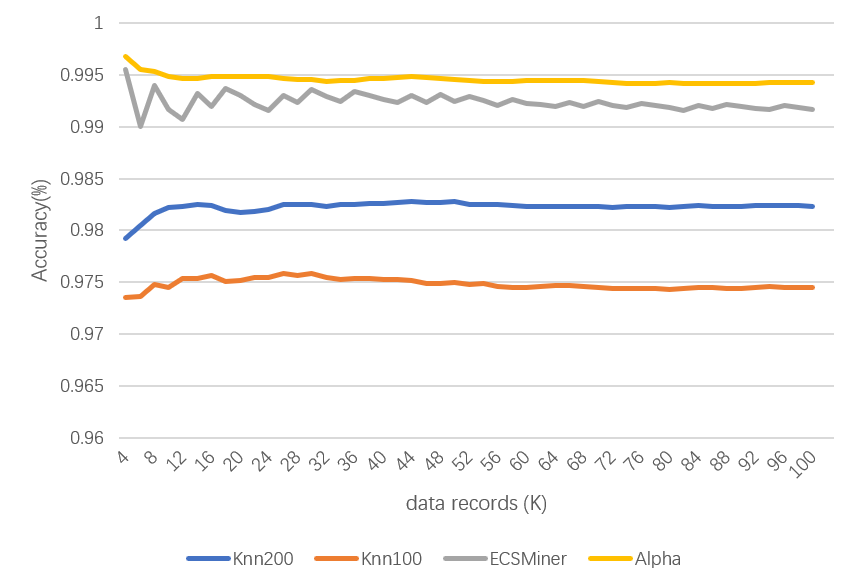
\includegraphics[width=1.0\textwidth]{figure-accuracy}
			\caption{Accuracy w.r.t. \# of records}
			\label{fig:accuracy}
		\end{minipage}
		\hspace{3mm}
		\begin{minipage}[t]{0.46\textwidth}
			\centering
			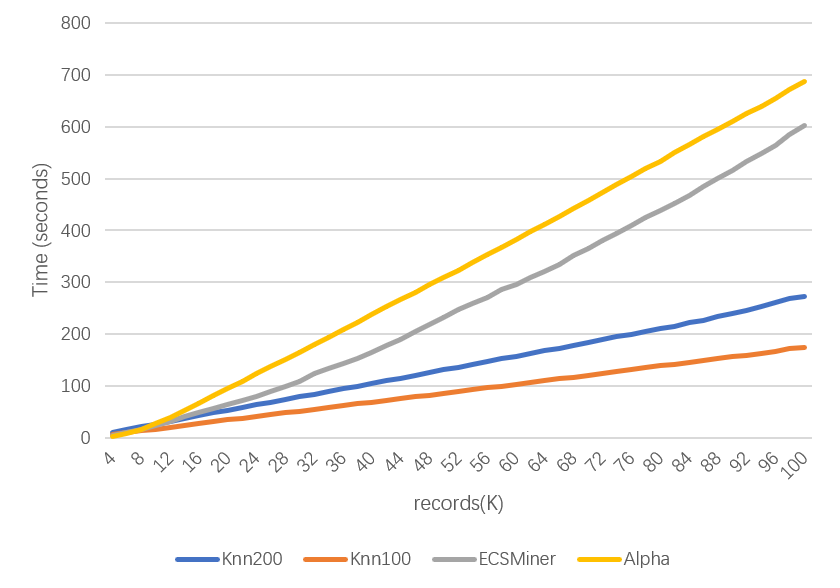
\includegraphics[width=1.0\textwidth]{figure-time}
			\caption{Time w.r.t. \# of records}
			\label{fig:time}
		\end{minipage}%
	\end{figure}
	
	Figure~\ref{fig:accuracy} shows the accuracy of different algorithms. We can see that our algorithm has the best performance. Since our method group the records with same label together, this can help to identify classes with small number of records. Both our method and ECSMiner have better performance than kNN. This is because kNN can be easily influenced by outliers in the data stream.
	
	Figure~\ref{fig:time} gives the time consumption. Among these methods, kNN has the minimum time consumption, since for each incoming data record, only the records that hold in the fixed size window need to be calculated. But when the window size becomes larger, the time kNN consumes goes larger as well. It's worth noticing that although our method perform better than ECSMiner in accuracy, we have slightly higher time consumption. This because we are treating different label separately during clustering, more iterations are introduced in this phase.
	
	
	\subsubsection{Varying $w$}
	\begin{figure}
		\centering
		\begin{minipage}[t]{0.46\textwidth}
			\centering
			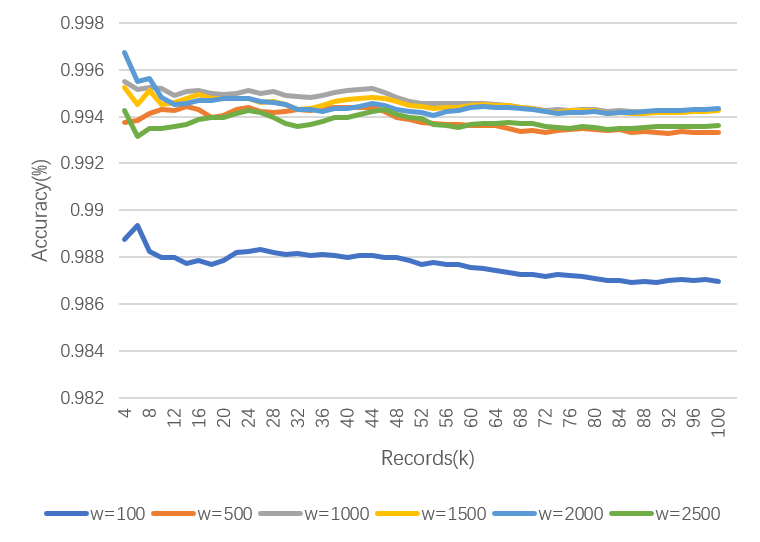
\includegraphics[width=1.0\textwidth]{figure-w-accuracy}
			\caption{Accuracy with different $w$}
			\label{fig:accuracy:w}
		\end{minipage}
		\hspace{3mm}
		\begin{minipage}[t]{0.46\textwidth}
			\centering
			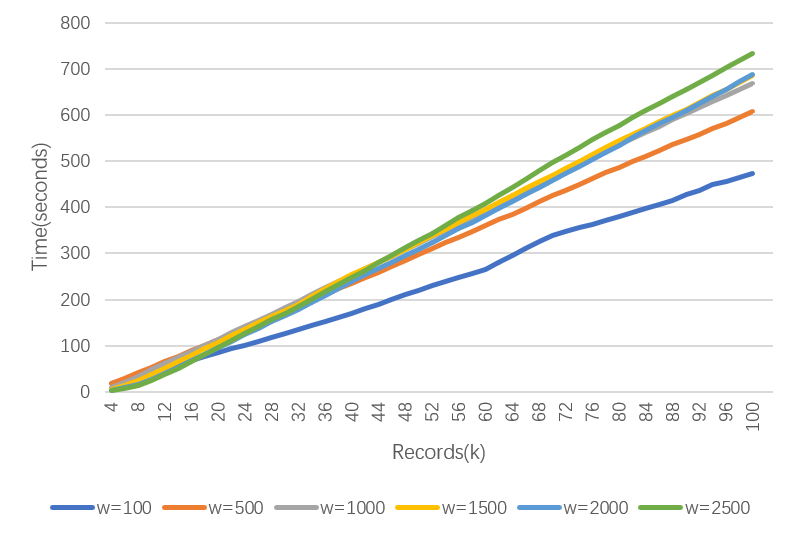
\includegraphics[width=1.0\textwidth]{figure-w-time}
			\caption{Time with different $w$}
			\label{fig:time:w}
		\end{minipage}%
	\end{figure}
	
	Figure~\ref{fig:accuracy:w} and ~\ref{fig:time:w} show the accuracy and time consumption with varying $w$ separately. Too small $w$ can lead to poor performance, but it can also speed up the algorithm. After some fixed value, $w$ won't influence much on both the performance and time consumption. This is because larger $w$ means less clustering times, meanwhile, the number of records that clustering method needs to process also increases. 
	
	\subsubsection{Varying $k$}
	
	In comparison, different values of $k$ have less influence on both accuracy and time. Figure~\ref{fig:accuracy:k} shows that larger $k$ values may lead to a worse accuracy at the beginning, but eventually, the overall performance won't differ much. Since $k$ value only being used in classification phase. When the number of total records is small, a smaller $k$ value would give us  better classification results.
	
	\begin{figure}
		\centering
		\begin{minipage}[t]{0.46\textwidth}
			\centering
			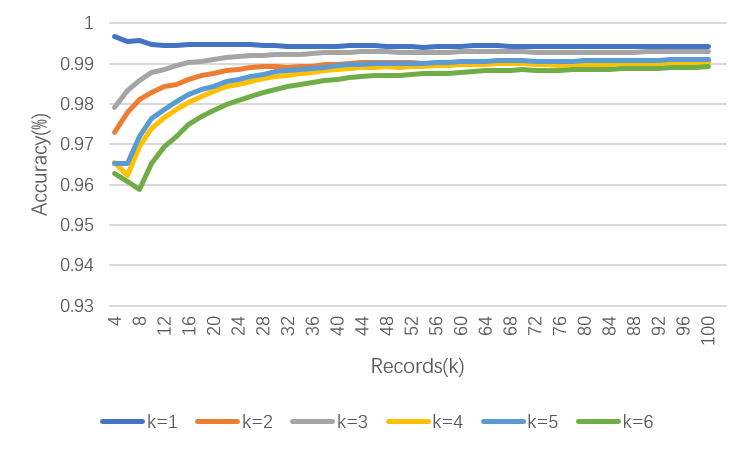
\includegraphics[width=1.0\textwidth]{figure-k-accuracy}
			\caption{Accuracy with different $k$}
			\label{fig:accuracy:k}
		\end{minipage}
		\hspace{3mm}
		\begin{minipage}[t]{0.46\textwidth}
			\centering
			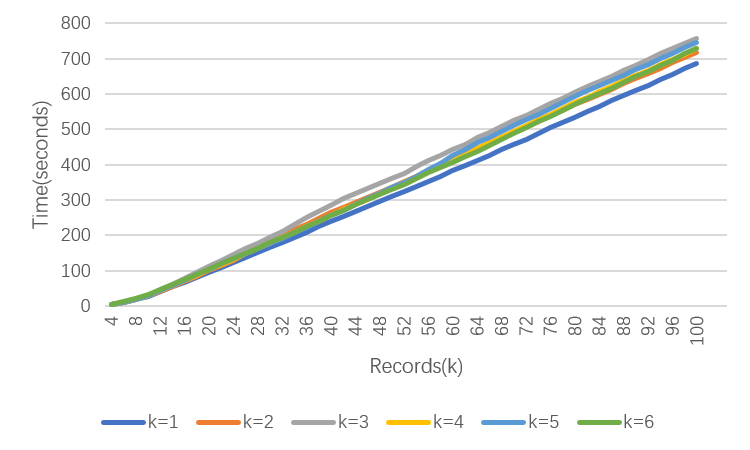
\includegraphics[width=1.0\textwidth]{figure-k-time}
			\caption{Time with different $k$}
			\label{fig:time:k}
		\end{minipage}%
	\end{figure}
	\subsubsection{Varying $c$}
	Different $c$ values means different number of clusters during point reducing phase. Smaller $c$ values can lead to faster speed during running, this can be verified from figure~\ref{fig:time:c}. Figure~\ref{fig:accuracy:c} shows that if $c$ is too small, the accuracy could be very poor. This is because small $c$ value means less points after clustering. Since we're grouping records with same label together, some critical points in those labels which have larger number of records may be discarded. Classification result can be highly influenced by points in other labels. After a certain threshold, $c$ value won't influence much on accuracy.
	\begin{figure}
		\centering
		\begin{minipage}[t]{0.46\textwidth}
			\centering
			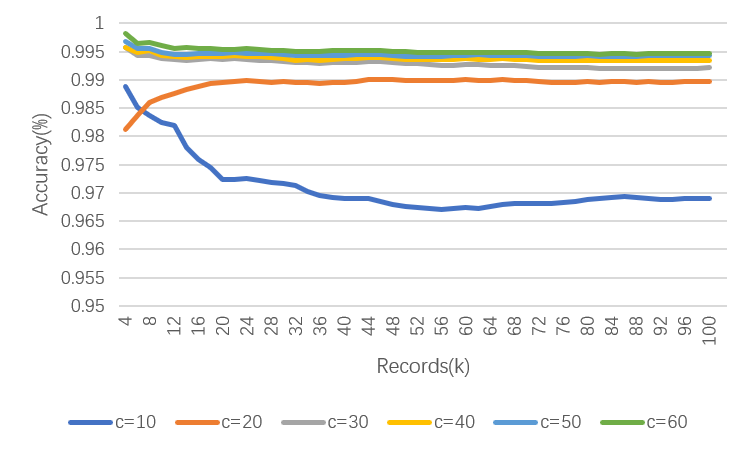
\includegraphics[width=1.0\textwidth]{figure-c-accuracy}
			\caption{Accuracy with different $c$}
			\label{fig:accuracy:c}
		\end{minipage}
		\hspace{3mm}
		\begin{minipage}[t]{0.46\textwidth}
			\centering
			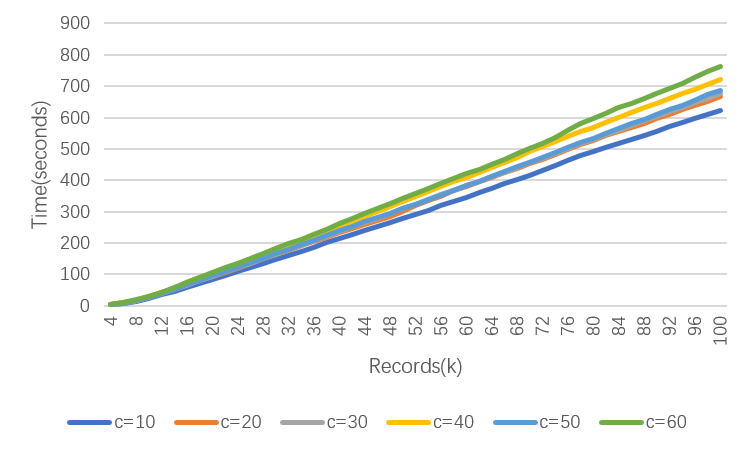
\includegraphics[width=1.0\textwidth]{figure-c-time}
			\caption{Time with different $c$}
			\label{fig:time:c}
		\end{minipage}%
	\end{figure}
	\subsubsection{Varying $N$}
	Figure~\ref{fig:accuracy:n} shows that smaller the number of partitions we hold in memory, worse the accuracy is. $N$ can be regard as one of the most important parameters in this algorithm, since it can have big impacts on time consumption (figure~\ref{fig:time:n}). Normally, $N$ should be chosen according to different scenarios. Large $N$ can lead to slow adaption phases, while algorithm with small $N$ value can be highly adapted to data drift.
	
	\begin{figure}
		\centering
		\begin{minipage}[t]{0.46\textwidth}
			\centering
			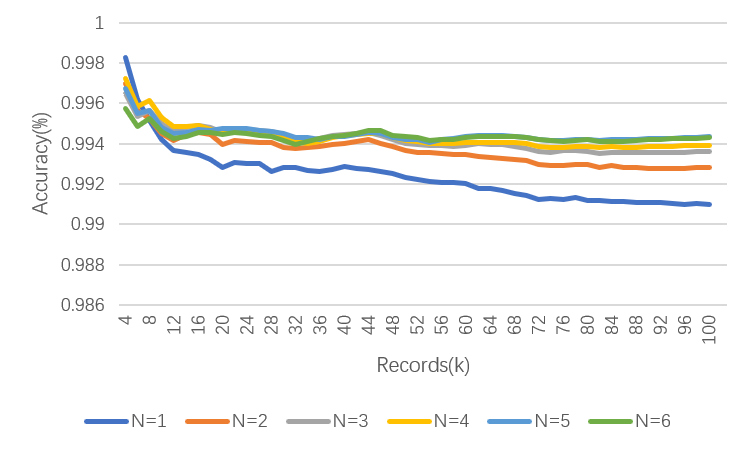
\includegraphics[width=1.0\textwidth]{figure-n-accuracy}
			\caption{Accuracy with different $N$}
			\label{fig:accuracy:n}
		\end{minipage}
		\hspace{3mm}
		\begin{minipage}[t]{0.46\textwidth}
			\centering
			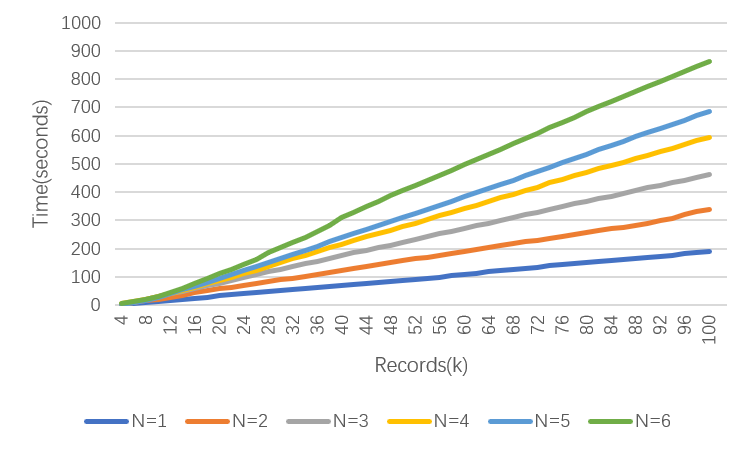
\includegraphics[width=1.0\textwidth]{figure-n-time}
			\caption{Time with different $N$}
			\label{fig:time:n}
		\end{minipage}%
	\end{figure}
	\section{Conclusion and Future Works} \label{conclusion}
	
	\subsection{Conclusion}
	In this paper, we present an online network intrusion detection system. Moreover, an online learning algorithm is given to classify incoming data records. Our method combines kNN and KMeans++ algorithms. We use kNN to make classification while using kMeans++ to clustering raw data records to reduce the total number of points. Through experiments, we can see that our method has better accuracy than ECSMiner, but takes longer time. Time consumption can be reduced by choosing different parameters. A influence of varying values for different parameters are given in the experiment analysis, which can be helpful for choosing parameter values in different scenarios.
	
	In general, most of the data mining algorithms are using one model to train and classify records with different labels. In our algorithm, we treat records with different labels separately, and use clustering method to reduce influence of outliers. This process can be regard as model ensemble. In stream data mining, since we want to learn most recent records incrementally, ensemble models can be very useful.
	
	\subsection{Future Works}
	We believe that there are still many problems can be addressed in online intrusion detection systems. Future works can be done in the following direction:
	\begin{enumerate}
		\item Speed improvement. Based on this paper, stream clustering methods, such as StreamKM++\cite{Ackermann2012}, CluStream can further applied. Stream clustering methods usually take less time than traditional methods. New data structure and techniques can also be introduced to speed up the whole process.
		\item Accuracy improvement. We can see from the experiments although only kNN and kMeans are applied, we can get good results. Introducing more complex data mining algorithms may have a better accuracy.
		\item Hybrid online learning methods. We can notice that two algorithms are used in this paper. To deal with data streams, trade-offs need to be made to deal with different aspect of problems. Hybrid methods are especially useful in dealing with such scenarios. Different strategies of combining methods is also another topic that worth study.
		\item Stream data preprocessing. Preprocessing can also have influence on the final result. How to extract attributes online, and how to perform adaptive normalization methods are also key issues in online learning scenarios.
		\item Handling delayed feedback. In our system, we make the assumption that a correct label of the record can be obtained right after the classification process completes. However, in real-world applications, feedback is less immediate and forthcoming. Different strategies for handling these delays and missing labels as well as the impact on accuracy and performance of the algorithm should be explored.
	\end{enumerate}

	\bibliographystyle{splncs03}
	\bibliography{reference}  
	
	\appendix
	\section{Appendix} \label{appendix}
	\subsection{Dataset}
	The KDDCup'99 dataset contains several data files. The one we used in our experiments named $kddcup.data\_10\_percent.gz$. Online dataset can be found through the following link:
	
	http://archive.ics.uci.edu/ml/machine-learning-databases/kddcup99-mld/
	
	\subsection{Programs}
	We implemented the experiments in python. The project contains two main modules:
	\begin{enumerate}
		\item \textit{tools}. This module contains preprocessing codes such as: normalization, feature selection, and result analysis tools.
		\item \textit{dmproject}. This module contains the implementation of our method ($alpha_kmeans.py$), ECSMiner ($ecsminer.py$) and windowed k-NN method($knn.py$). Most of the parameters can be changed with input values.
	\end{enumerate}
\end{document}